\chapter{Analyse et recommandations}
\label{chap:4}
\sloppy

\section{Analyse des cas de succès et d'échec}

Dans l'ensemble, il a été observé qu'une classe, à savoir \textbf{AFV}  a bien fonctionné dans nos deux expériences.
La raison en est que cette classe avait plus de données d'entraînement que les autres classes.
Les détails de notre ensemble de données proposé sont donnés dans le tableau \ref{tab:label_data}.
Au cours de l'analyse, nous avons observé que le système avait de bonnes performances sur les cas de test avec des véhicules visibles, mais il y avait des difficultés dans certains cas pour lesquels nous avions un petit jeu de données d'entraînement.
Il fonctionne bien sur les véhicules militaires dans les données non vues par rapport aux autres véhicules militaires car le rapport entre ses données d'entraînement est plus élevé.

Le modèle commence à mal fonctionner sur certaines données. Cela est dû au fait qu'il y a moins de données d'entraînement par rapport aux autres classes.

\begin{table}[H]
    \centering
    \begin{tabular}{|l|l|l|p{2.8cm}|p{2cm}|p{2cm}|p{2cm}|}
        \hline
        \textbf{Label} & \textbf{Quantité} & \textbf{Pourcentage} & \textbf{Modèles} & \textbf{Précision moyenne} & \textbf{Recall moyen} & \textbf{F1-Score moyen} \\ \hline
        AFV            & 6694              & 82.5\%               & YoloV8 (m et l)  & 0.71                       & 0.676                 & 0.69                    \\ \hline
        APC            & 1212              & 15.0\%               & YoloV8 (m et l)  & 0.58                       & 0.544                 & 0.557                   \\ \hline
        LAV            & 374               & 4.6\%                & YoloV8 (m et l)  & 0.52                       & 0.464                 & 0.49                    \\ \hline
        MEV            & 123               & 1.5\%                & YoloV8 (m et l)  & 0.29                       & 0.530                 & 0.374                   \\ \hline
    \end{tabular}
    \caption{Tableau des moyennes des résultats}
    \label{tab:label_data}
\end{table}


\section{Limites et perspectives}
\subsection{Modèle de détection d'objets}

Le modèle  \textbf{YoloV8}, grâce à plusieurs contributions, a connu un gain de performance considérable ces dernières années.
Nous avons des scores de précision d'environ 80\% malgré la faible quantité de données utilisée pour l'entraînement du modèle.
Néanmoins, les paramètres (hyperparamètres) de ces modèles deviennent plus complexes à comprendre et à personnaliser pour améliorer les résultats et les adapter à nos besoins.
À ce jour, par rapport à nos contraintes en détection de véhicules militaires, YoloVx est le modèle de détection le plus performant.
Nous allons continuer à ajuster les paramètres pour obtenir un modèle encore plus performant.

\subsection{Augmentation des données}
\subsubsection{Transformation des images}
\label{trando_image}
Dans le cadre de cette étude, nous avons appliqué les transformations telles que le \textit{scaling}, le \textit{XYMasking}, et des transformations liées aux conditions météorologiques.
Ces techniques ont permis de presque doubler le nombre d'images et leurs annotations pour l'entraînement de notre modèle.

Après un contrôle de qualité des images, nous avons constaté qu'il y a des images floues ou mal exploitées illisibles.
Le tri de ces images n'est pas envisageable compte tenu de la quantité (3335) d'images du jeu de données sur lesquelles les transformations ont été appliquées.

\begin{figure}[H]
    \centering
    \begin{subfigure}[b]{0.4\textwidth}
        \centering
        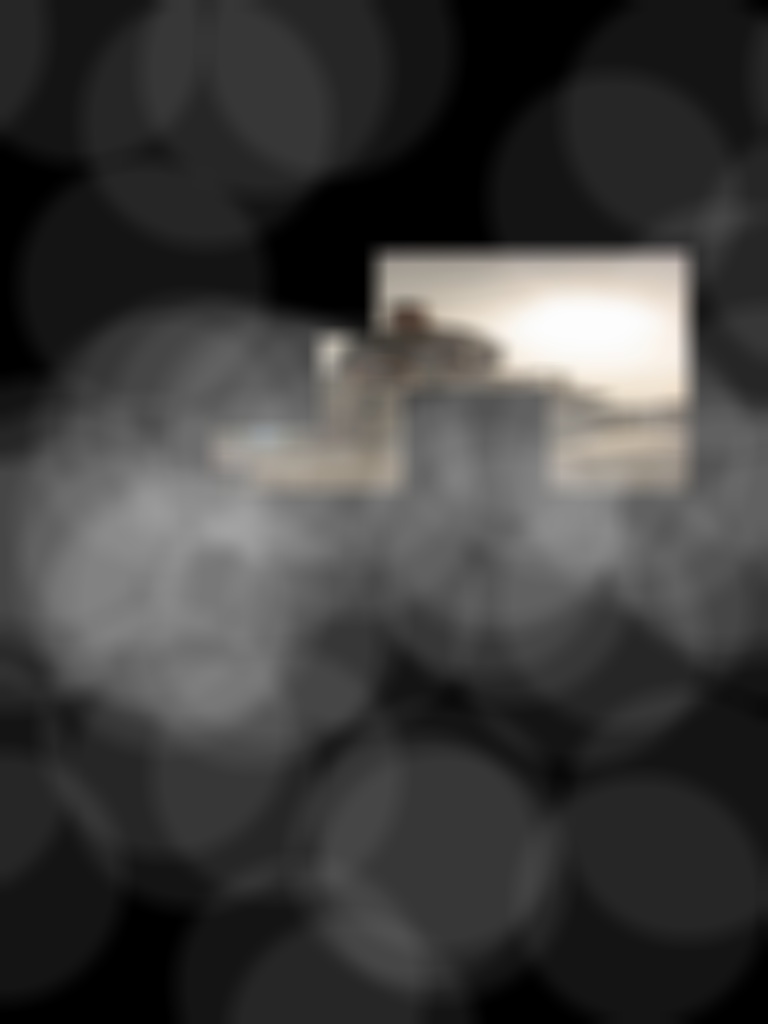
\includegraphics[width=0.8\textwidth]{./images/augmented-1.jpg}
    \end{subfigure}
    \hfill
    \begin{subfigure}[b]{0.4\textwidth}
        \centering
        
\includegraphics[width=\textwidth]{./images/augmented-2.jpg}
    \end{subfigure}
    \vskip\baselineskip
    \begin{subfigure}[b]{0.4\textwidth}
        \centering
        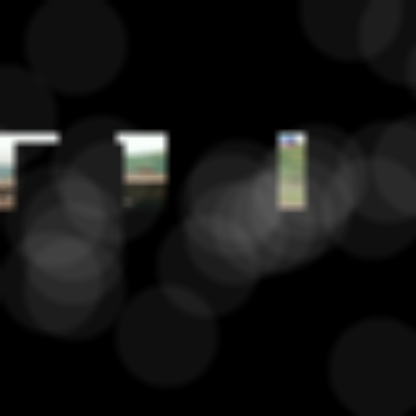
\includegraphics[width=0.8\textwidth]{./images/augmented-3.jpg}
    \end{subfigure}
    \hfill
    \begin{subfigure}[b]{0.4\textwidth}
        \centering
        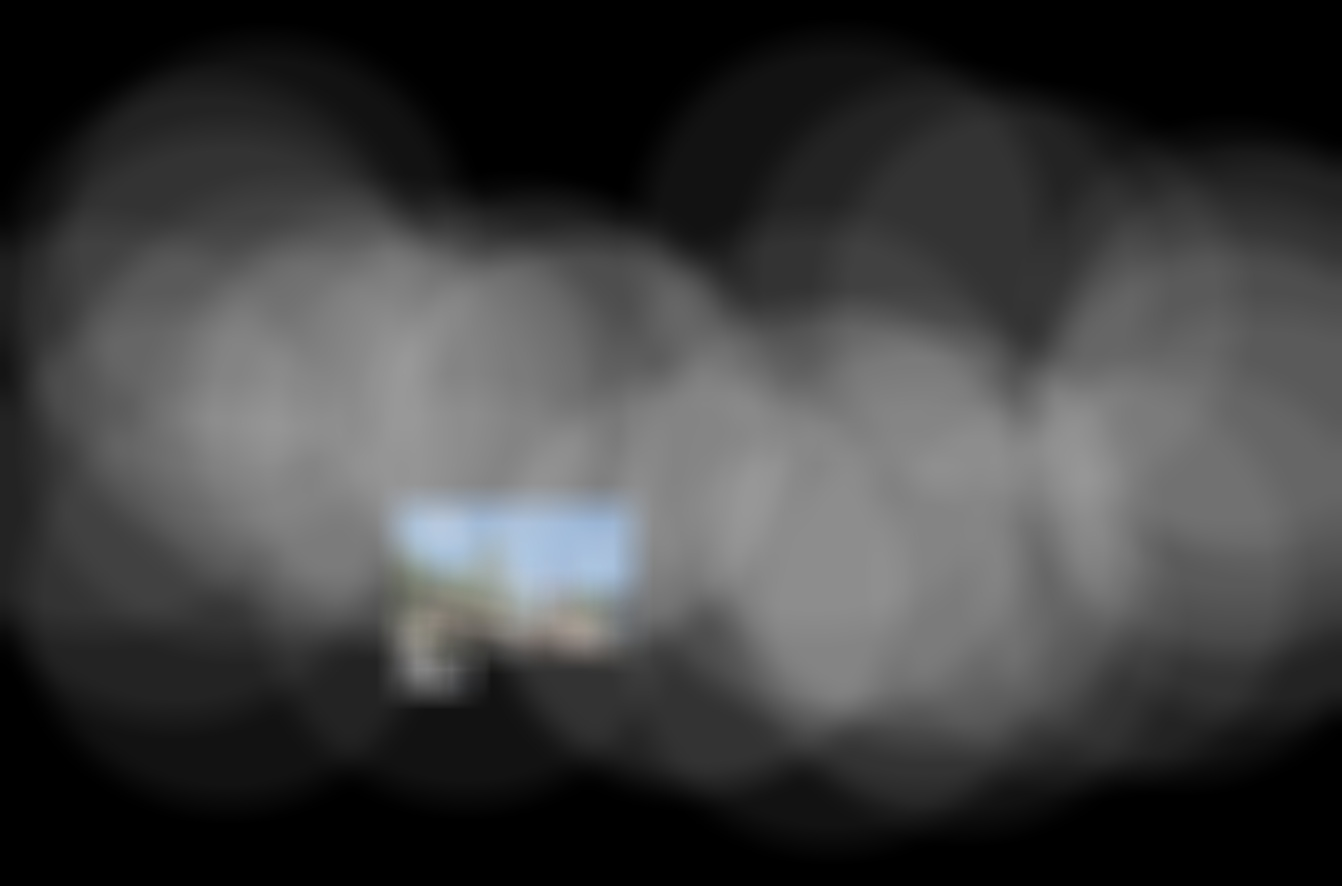
\includegraphics[width=\textwidth]{./images/augmented-4.JPEG}
    \end{subfigure}
    \caption{Exemples d'images transformées de véhicules militaires inexploitables}
    \label{fig:image_floues}
\end{figure}

\subsubsection{Génération d'images}

La génération d'images nous permet d'augmenter le nombre de véhicules de notre jeu de données.
Comme inconvénients, nous pouvons citer :

\begin{itemize}
    \item Elle ne peut générer qu'un seul type de véhicule.
    \item Beaucoup d'images ne sont pas réalistes et sont donc inexploitables.
    \item Les images ne sont pas annotées et nécessitent une annotation manuelle.
    \item Aucun moyen d'évaluer objectivement la qualité du rendu. Tout est subjectif, ce qui rend l'évaluation fastidieuse.
\end{itemize}

\begin{quotation}
    \textit{If you are going for a certain result in your art, then determining if a model is over or under trained is always going to be subjective, because art is subjective.\cite{reddit_proverbe}}
\end{quotation}

\begin{figure}[H]
    \centering
    \begin{subfigure}[b]{0.45\textwidth}
        \centering
        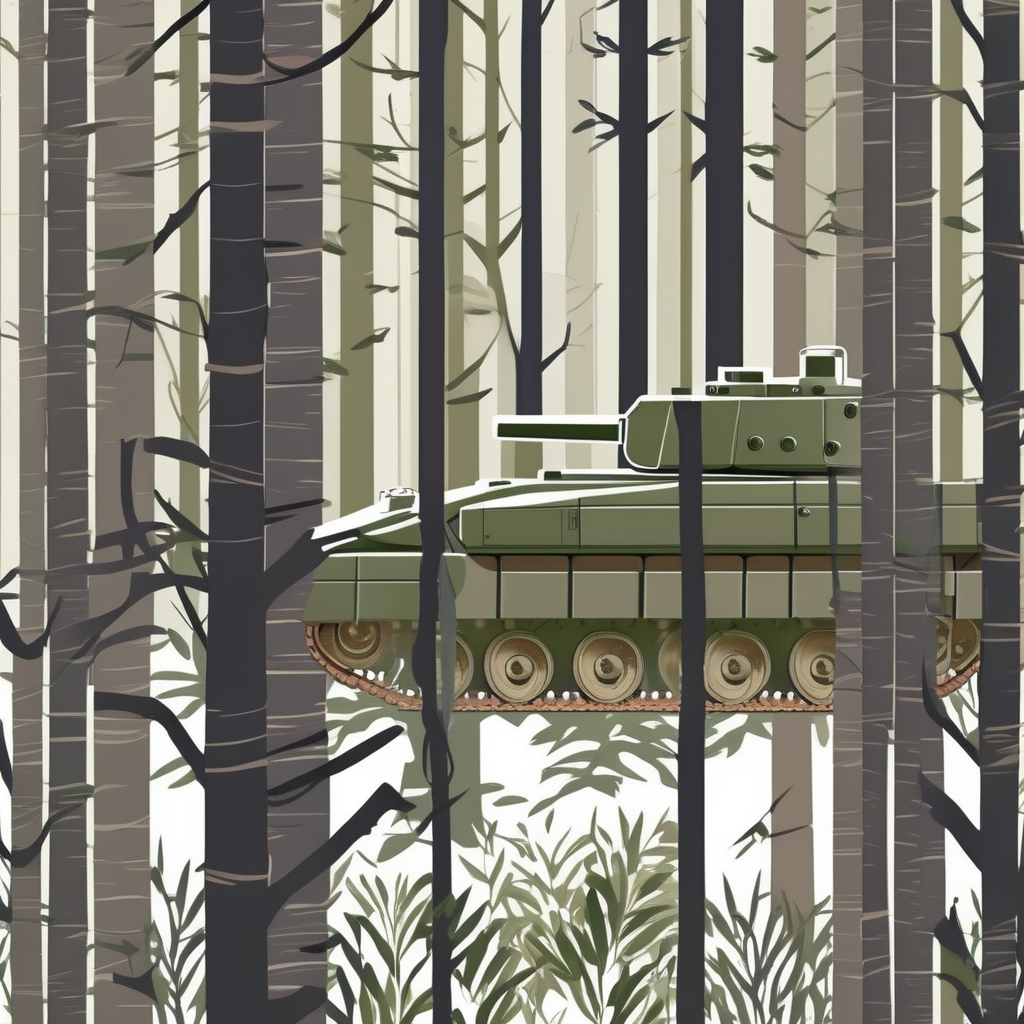
\includegraphics[width=0.8\textwidth]{./images/tank-forest_camouflage-1.png}
    \end{subfigure}
    \hfill
    \begin{subfigure}[b]{0.45\textwidth}
        \centering
        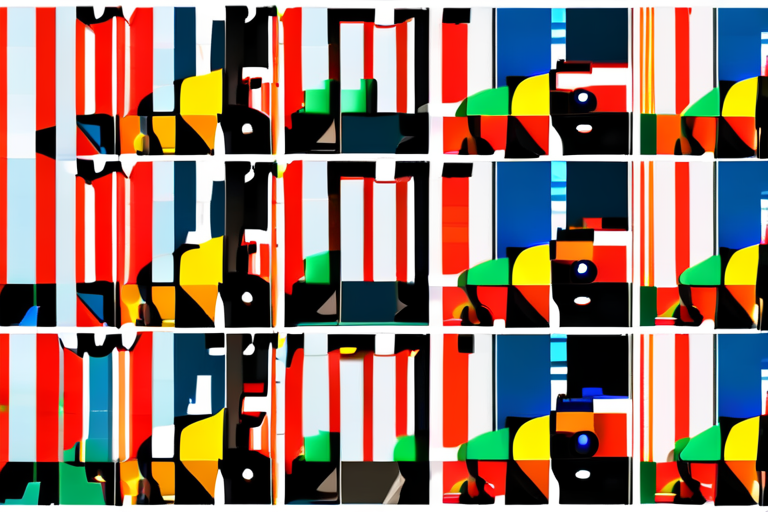
\includegraphics[width=\textwidth]{./images/tank-night_operation-1.png}
    \end{subfigure}
    \vskip\baselineskip
    \begin{subfigure}[b]{0.45\textwidth}
        \centering
        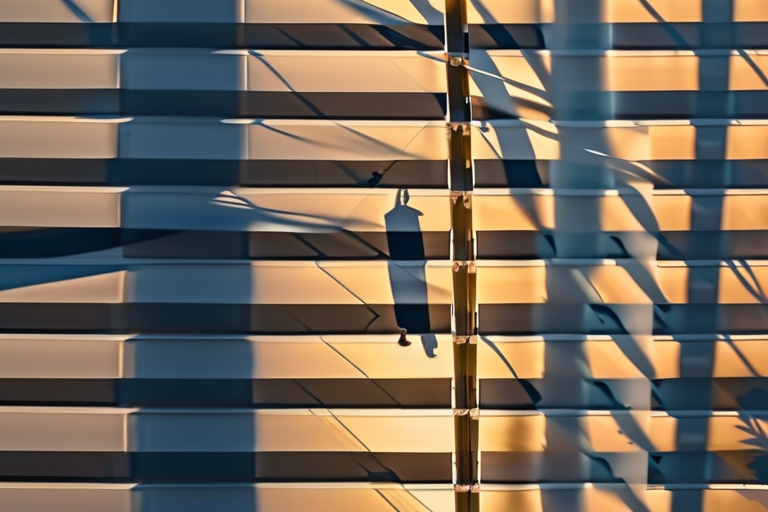
\includegraphics[width=\textwidth]{./images/tank-sunrise_maneuver-1.png}
    \end{subfigure}
    \hfill
    \begin{subfigure}[b]{0.45\textwidth}
        \centering
        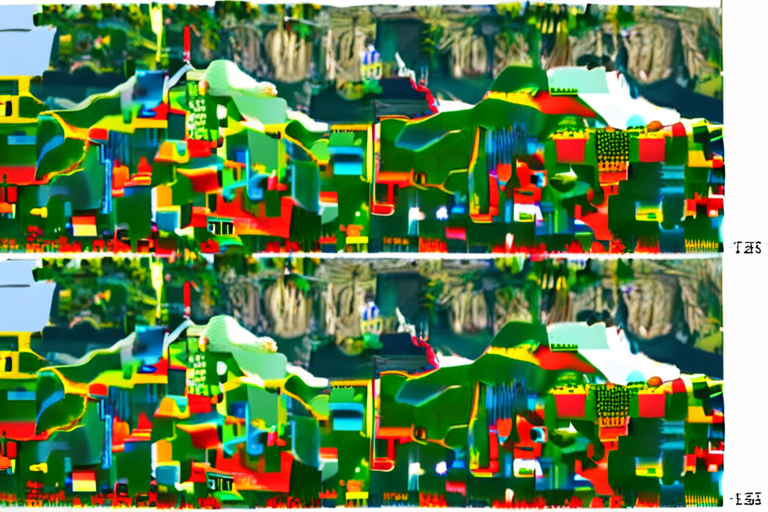
\includegraphics[width=\textwidth]{./images/tank-mountain_path-0.png}
    \end{subfigure}
    \caption{Exemples d'images synthétiques de véhicules militaires irréalistes et inexploitables}
\end{figure}


\subsection{Évolution des résultats}

Les résultats obtenus avec les techniques de \textit{data augmentation} ont révélé une dégradation significative des performances.
Par exemple, avec les données augmentées, le \textit{mAP} a chuté de \textbf{0.66} à \textbf{0.34}, et les scores F1 pour certaines classes ont diminué de manière notable (voir Tableaux \ref{tab:map-train-01} et \ref{tab:results_moy_prepare03}).
Cela montre que les transformations appliquées n'ont pas eu l'effet escompté sur les performances du modèle.


\newcolumntype{C}[1]{>{\centering\arraybackslash}p{#1}}

\begin{table}[H]
    \centering
    \begin{tabular}{|C{1.5cm}|C{1.8cm}|C{1.5cm}|C{2cm}|C{1.8cm}|C{1.5cm}|C{2cm}|}
        \hline
        \multirow{2}{*}{\textbf{Classes}} & \multicolumn{3}{c|}{\textbf{Sans data augmentation}} & \multicolumn{3}{c|}{\textbf{Avec data augmentation}}                                                                                             \\ \cline{2-7}
                                          & \textbf{Précision}                                   & \textbf{Recall}                                      & \textbf{F1-score} & \textbf{Précision}    & \textbf{Recall}       & \textbf{F1-score}     \\ \hline
        AFV                               & \textbf{0.76}                                        & \textbf{0.85}                                        & \textbf{0.80}     & \textcolor{red}{0.71} & \textcolor{red}{0.66} & \textcolor{red}{0.68} \\ \hline
        APC                               & \textbf{0.69}                                        & \textbf{0.72}                                        & \textbf{0.70}     & \textcolor{red}{0.59} & \textcolor{red}{0.57} & \textcolor{red}{0.58} \\ \hline
        LAV                               & \textbf{0.55}                                        & \textbf{0.72}                                        & \textbf{0.62}     & \textcolor{red}{0.51} & \textcolor{red}{0.41} & \textcolor{red}{0.46} \\ \hline
        MEV                               & \textbf{0.62}                                        & \textbf{0.71}                                        & \textbf{0.67}     & \textcolor{red}{0.22} & \textcolor{red}{0.40} & \textcolor{red}{0.29} \\ \hline
        \textbf{mAP}                      & \multicolumn{3}{c|}{\textbf{0.6609}}                 & \multicolumn{3}{c|}{\textcolor{red}{0.3425}}                                                                                                     \\ \hline
    \end{tabular}
    \caption{Comparaison des résultats sans et avec data augmentation}
    \label{tab:comparaison_aug}
\end{table}

\subsubsection{Analyse des résultats}

Il a été observé que certaines transformations d'image, telles que l'ajout de brouillard, ont altéré la qualité des images, rendant ces dernières inutilisables pour l'entraînement du modèle  (Ex. Figures \ref{fig:image_floues}).
Ces images floues ont fortement perturbé le modèle, réduisant sa capacité à reconnaître correctement les objets.
Ce phénomène s'est particulièrement manifesté pour les classes \textbf{MEV} et \textbf{LAV}, où les performances ont chuté de manière notable.\\


\subsubsection{Hypothèses et solutions envisageables :}

\begin{itemize}
    \item Revoir les paramètres des transformations appliquées, notamment en réduisant l’intensité ou la fréquence d’apparition des effets de brouillard.
    \item Retirer certaines transformations spécifiques (comme le brouillard) afin de tester si elles ont un impact négatif sur les performances.
    \item Générer des images augmentées avec des transformations moins agressives tout en conservant la diversité des conditions environnementales.
    \item Trier manuellement les images augmentées pour écarter celles qui sont inutilisables.
\end{itemize}

\section{Recommandations}

En tenant compte des résultats et des limites identifiées, nous proposons quelques pistes d'amélioration :

\begin{itemize}
    \item \textbf{Transformation d'images :} Nous recommandons de limiter les transformations à deux types par image au lieu de trois. Cela réduirait la probabilité d'obtenir des images complètement floues et inexploitables. De plus, cela permettrait de produire plusieurs combinaisons de transformations, augmentant ainsi la taille du jeu de données.
    \item \textbf{Images synthétiques :} Stable Diffusion V3 et XL semblent générer des images moins réalistes que la version 1.5. Il serait intéressant de se concentrer sur cette version avant de passer aux versions plus récentes.
    \item \textbf{Jeux vidéos :} Explorer la possibilité d'extraire des images de véhicules militaires à partir de jeux vidéos.
    \item \textbf{Films d'action/guerre :} En plus d'avoir des images réalistes, nous pourrions obtenir plusieurs images dans des situations complexes (camouflage, explosion, etc.). Développer un outil permettant d'extraire des séquences vidéo contenant des scènes de guerre afin d'obtenir un maximum d'images.
    \item \textbf{Vidéos des réseaux sociaux :} Scruter les publications pouvant contenir des images ou vidéos de véhicules militaires dans des situations complexes à reproduire.
\end{itemize}

Nous tenons à rester objectifs dans nos recommandations car les images issues de ce travail, en majorité, ne seront pas annotées et nécessiteront donc un travail supplémentaire d’annotation manuelle, qui est souvent très coûteux, notamment en termes de temps.
